\documentclass[12pt,a4paper]{article}
\usepackage[utf8]{inputenc}
\usepackage[T1]{fontenc}
\usepackage{times}
\usepackage[margin=2.5cm]{geometry}
\usepackage{setspace}
\onehalfspacing
\usepackage{graphicx}
\usepackage{booktabs}
\usepackage{hyperref}
\usepackage{amsmath}

\title{Temples Without Villages: Candi and the Hidden Settlement Geography of Volcanic Java}

\author{Mukhlis Amien\textsuperscript{1} \and Go Frendi Gunawan\textsuperscript{1}}

\date{}

\begin{document}

\maketitle

\noindent\textsuperscript{1}Lab Data Sains, Universitas Bhinneka Nusantara, Malang, Indonesia

\vspace{0.5em}
\noindent\textbf{Corresponding author:} Mukhlis Amien (\texttt{amien@ubhinus.ac.id})\\
\noindent ORCID: 0000-0002-1848-167X

\begin{abstract}
Java's volcanic landscape has buried centuries of human settlement beneath pyroclastic debris.
We argue that surviving Hindu-Buddhist temples (\emph{candi}) mark the locations of these lost communities.
Spatial analysis of 142 candi reveals systematic clustering on western volcanic flanks---the zones most intensely buried by lahars and tephra---while temple orientation follows religious prescription.
Georeferenced inscriptions occupy a different spatial zone, clustering 15--30~km from volcanoes where royal courts operated.
This divergence reveals two distinct geographies: a sacred landscape on volcanic slopes and an administrative landscape on alluvial plains.
The 929~CE Mataram collapse provides a before-after observation confirming this spatial structure, and the 2008 discovery of a buried village at Liangan demonstrates the model's plausibility.
Pre-modern Java was far more extensively settled than the surviving record suggests.
\end{abstract}

\vspace{0.5em}
\noindent\textbf{Keywords:} Java, candi, volcanic taphonomy, settlement geography, inscriptions, Hindu-Buddhist archaeology, Insulindia, buried landscapes


\newpage

% ============================================================
\section{Introduction: What Survives and What is Lost}
% ============================================================

The scholarly understanding of pre-modern Java rests on what the island's volcanic landscape has permitted to survive.
Lombard's magisterial portrait of the ``Javanese crossroads'' drew upon inscriptions, temple complexes, and literary texts---all products of elite patronage, all rendered in durable media.\footnote{Denys Lombard, \emph{Le carrefour javanais: essai d'histoire globale}, 3 vols.\ (Paris: \'{E}ditions de l'\'{E}cole des hautes \'{e}tudes en sciences sociales, 1990).}
His three-volume synthesis demonstrated how Java functioned as a crossroads of Indian, Chinese, Islamic, and European cultural currents.
Yet Lombard himself was aware that this portrait was drawn almost entirely from the records of courts and religious institutions---the very sources most likely to survive in durable media.
The villages, markets, workshops, and domestic spaces that constituted the lived experience of the vast majority of Javanese---built in wood, bamboo, and thatch---have left almost no archaeological trace.

Lombard's third volume, \emph{Les r\'{e}seaux}, traced the commercial and cultural networks that converged on Java, but beneath these layers of Indian, Chinese, and Islamic influence he repeatedly acknowledged a deeper stratum: the \emph{monde du village}, the Austronesian substrate of rice cultivation, ancestor worship, and communal organisation that persisted through every successive wave of external contact.\footnote{Lombard, \emph{Le carrefour javanais}, vol.~3, esp.\ chap.~9--10 on the persistence of village structures beneath successive ``r\'{e}seaux.''}
Yet this foundational layer is almost entirely absent from the documentary record that Lombard himself relied upon.
The very sources that made his synthesis possible---court inscriptions, temple reliefs, Chinese trade records---are products of the elite networks, not of the villages.
The volcanic landscape of Java offers a material explanation for this silence.

This evidential asymmetry is not accidental.
Java hosts 34 active volcanoes that have been burying the landscape at measurable rates for millennia.
When Wolters described the ``localization'' of Indic culture in Southeast Asia---the creative process by which imported cultural elements were absorbed and transformed by local societies---he worked primarily from inscriptions and temples.\footnote{O.~W.\ Wolters, \emph{History, Culture, and Region in Southeast Asian Perspectives}, rev.\ ed.\ (Ithaca: Cornell University Southeast Asia Program, 1999).}
His framework of localisation implied an active indigenous substrate that selected, adapted, and reinterpreted external influences.
But the material evidence of that substrate---the domestic architecture, the organic-media records, the vernacular religious practices---has been systematically subtracted from the evidential base by the very geological processes that made Java's soils so productive.

Miksic has noted the paradox directly: Java's archaeological record is simultaneously one of the richest in Southeast Asia in monumental terms and one of the most incomplete in settlement terms.\footnote{John~N.\ Miksic, ``The Classical Cultures of Indonesia,'' in \emph{Southeast Asia: From Prehistory to History}, ed.\ Ian Glover and Peter Bellwood (London: RoutledgeCurzon, 2004), 234--256.}
De Casparis, mapping the distribution of inscriptions across Java, observed that they clustered in areas associated with court activity---the Kedu plain, the Prambanan basin, the Brantas valley---while the volcanic highlands remained ``comparatively inscription-free.''\footnote{J.~G.\ de Casparis, \emph{Indonesian Palaeography: A History of Writing in Indonesia from the Beginnings to c.~A.D.~1500} (Leiden: E.~J.\ Brill, 1975).}
This clustering has traditionally been interpreted as reflecting the distribution of political power.
But it may equally reflect the distribution of a particular \emph{genre} of evidence: administrative texts produced by and for court institutions, in zones where volcanic burial was least severe.

This paper proposes that surviving candi can serve as witnesses---not merely to the religious life of Hindu-Buddhist Java, but to the geography of an entire buried settlement landscape.
By analysing where temples were built, where inscriptions were composed, and where these two categories of evidence diverge, we extract spatial information about past communities that no surface survey can now recover.
The argument proceeds in three stages: first, we establish the taphonomic mechanism by which volcanic sedimentation has erased the settlement record; second, we demonstrate that candi and inscriptions occupy systematically different spatial zones; and third, we show that the 929~CE political collapse provides a natural experiment confirming this spatial structure.

% ============================================================
\section{The Volcanic Landscape as Taphonomic Agent}
% ============================================================

Java lies on the Sunda Arc, where the Indo-Australian plate subducts beneath the Eurasian plate, producing one of the densest volcanic concentrations on Earth.
The island hosts 34 of Indonesia's 127 active volcanoes, erupting on average once every 1--2 years.\footnote{Global Volcanism Program, \emph{Volcanoes of the World}, v.~5.1.1 (Smithsonian Institution, 2023), \url{https://volcano.si.edu/}.} Throughout this paper, volcano locations follow the canonical 30-peak inventory of active and recently active Java volcanoes (Smithsonian GVP-derived), replacing the partial inventories used in earlier project work.
Merapi alone has produced more than 60 eruptions in the last millennium.\footnote{Christopher~G.\ Newhall et al., ``10,000 Years of Explosive Eruptions of Merapi Volcano, Central Java: Archaeological and Modern Implications,'' \emph{Journal of Volcanology and Geothermal Research} 100, no.~1--4 (2000): 9--50.}

The archaeological consequence is progressive burial.
Unlike the catastrophic single-event burial at Pompeii or Akrotiri, Java's temples and settlements were buried by cumulative deposition---repeated small to moderate events (lahars, tephra falls, pyroclastic surges) accumulating over centuries.\footnote{Franck Lavigne and Jean-Claude Thouret, ``Sediment Transportation and Deposition by Rain-Triggered Lahars at Merapi Volcano, Central Java, Indonesia,'' \emph{Geomorphology} 49, no.~1--2 (2003): 45--69.}
Measured sedimentation rates range from 2.4~mm/yr on distal slopes to 6.2~mm/yr on proximal flanks.
At these rates, a structure abandoned at ground level would be covered by 2.4--6.2~metres within a millennium---rendering it invisible to surface survey.

Colonial-era archaeologists documented the consequences directly.
The \emph{Oudheidkundig Verslag} reports of 1912--1929 record numerous instances of archaeological structures found at depth: temples near Kelud under 2~m of lahar deposit, Trowulan structures at 3.5--4.3~m, a Vi\d{s}\d{n}u statue at Prambanan at 9.14~m below the modern surface.\footnote{\emph{Oudheidkundig Verslag} (Batavia: Oudheidkundige Dienst in Nederlandsch-Indi\"{e}, 1912--1929). See also R.~W.\ van Bemmelen, \emph{The Geology of Indonesia}, vol.~1A (The Hague: Government Printing Office, 1949).}
The discovery of Candi Sambisari in 1966 at 6.5~m depth, and Candi Kimpulan in 2009 at 2.5~m, confirmed that significant Hindu-Buddhist structures can be completely concealed within centuries of abandonment.\footnote{Prishardoyo Bagyo Putra and Ayu Setyastuti, ``Le complexe cultuel de Kimpulan, site enfoui sous les cendres du Merapi (Yogyakarta, Java central),'' \emph{Bulletin de l'\'{E}cole fran\c{c}aise d'Extr\^{e}me-Orient} 105 (2019): 377--402.}

This taphonomic process is not random.
It preferentially erases evidence from the zones closest to volcanoes: the very areas that, in Mohr's analysis, supported the highest population densities due to the exceptional fertility of volcanic soils.\footnote{E.~C.~J.\ Mohr, ``The Relation between Soil and Population Density in the Netherlands East Indies,'' in \emph{Comptes Rendus du Congr\`{e}s International de G\'{e}ographie} (Amsterdam, 1938).}
The irony is precise: the geological process that made Java agriculturally productive has simultaneously buried the archaeological evidence of the civilisations that productivity sustained.


% ============================================================
\section{Sacred Geography: Mountains, Temples, and the Western Flank}
% ============================================================

\subsection{Candi as Settlement Witnesses}

Hindu-Buddhist candi---monumental structures of andesite and brick---resist volcanic burial and tropical weathering far better than organic-material settlements.
Of the 142 candi for which coordinates were compiled from published surveys, heritage registries, and standard catalogues,\footnote{Jacques Dumar\c{c}ay, \emph{The Temples of Java} (Oxford: Oxford University Press, 1993). R.\ Soekmono, \emph{The Javanese Candi: Function and Meaning} (Leiden: Brill, 1995).} most are visible at the surface today, and others were rediscovered through excavation---Sambisari in 1966 and Kimpulan in 2009, each buried for centuries before its discovery.
They are, in Schiffer's terminology, products of differential formation processes: what survives is what resists.\footnote{Michael~B.\ Schiffer, \emph{Formation Processes of the Archaeological Record} (Albuquerque: University of New Mexico Press, 1987).}

But candi were never isolated monuments.
Soekmono's study of candi function emphasised their role within settlement complexes---surrounded by villages, irrigated fields, markets, and craft production areas.
De Groot's spatial analysis of Central Javanese candi demonstrated that temples were oriented toward and clustered near major volcanoes, particularly Merapi and Penanggungan.\footnote{V\'{e}ronique~M.Y.\ de Groot, \emph{Candi, Space and Landscape: A Study on the Distribution, Orientation and Spatial Organization of Central Javanese Temple Remains} (PhD diss., Leiden University, 2009).}
A quantitative test of this co-location strengthens the claim: of 108 non-temple archaeological sites in East Java, 81\% lie within 10~km of the nearest candi, with a mean distance of 6.8~km.\footnote{Monte Carlo simulation ($p < 0.0001$, 10,000 permutations) confirms that the observed candi-settlement proximity cannot be explained by chance clustering.}
Candi and settlements are spatially co-located---confirming that temples genuinely mark the centres of broader settlement complexes.

\subsection{Western Flanks: Between Landscape and Cosmology}

Analysis of the bearing from each candi to its nearest active volcano reveals a striking pattern (Figure~\ref{fig:polar}).
The mean bearing is 298\textdegree{} (west-northwest), with nearly half of all candi (47.9\%) on western flanks; the eastern quadrant contains under 10\%.\footnote{Rayleigh test for circular non-uniformity: $p = 1.2 \times 10^{-9}$.}

\begin{figure}[h]
\centering
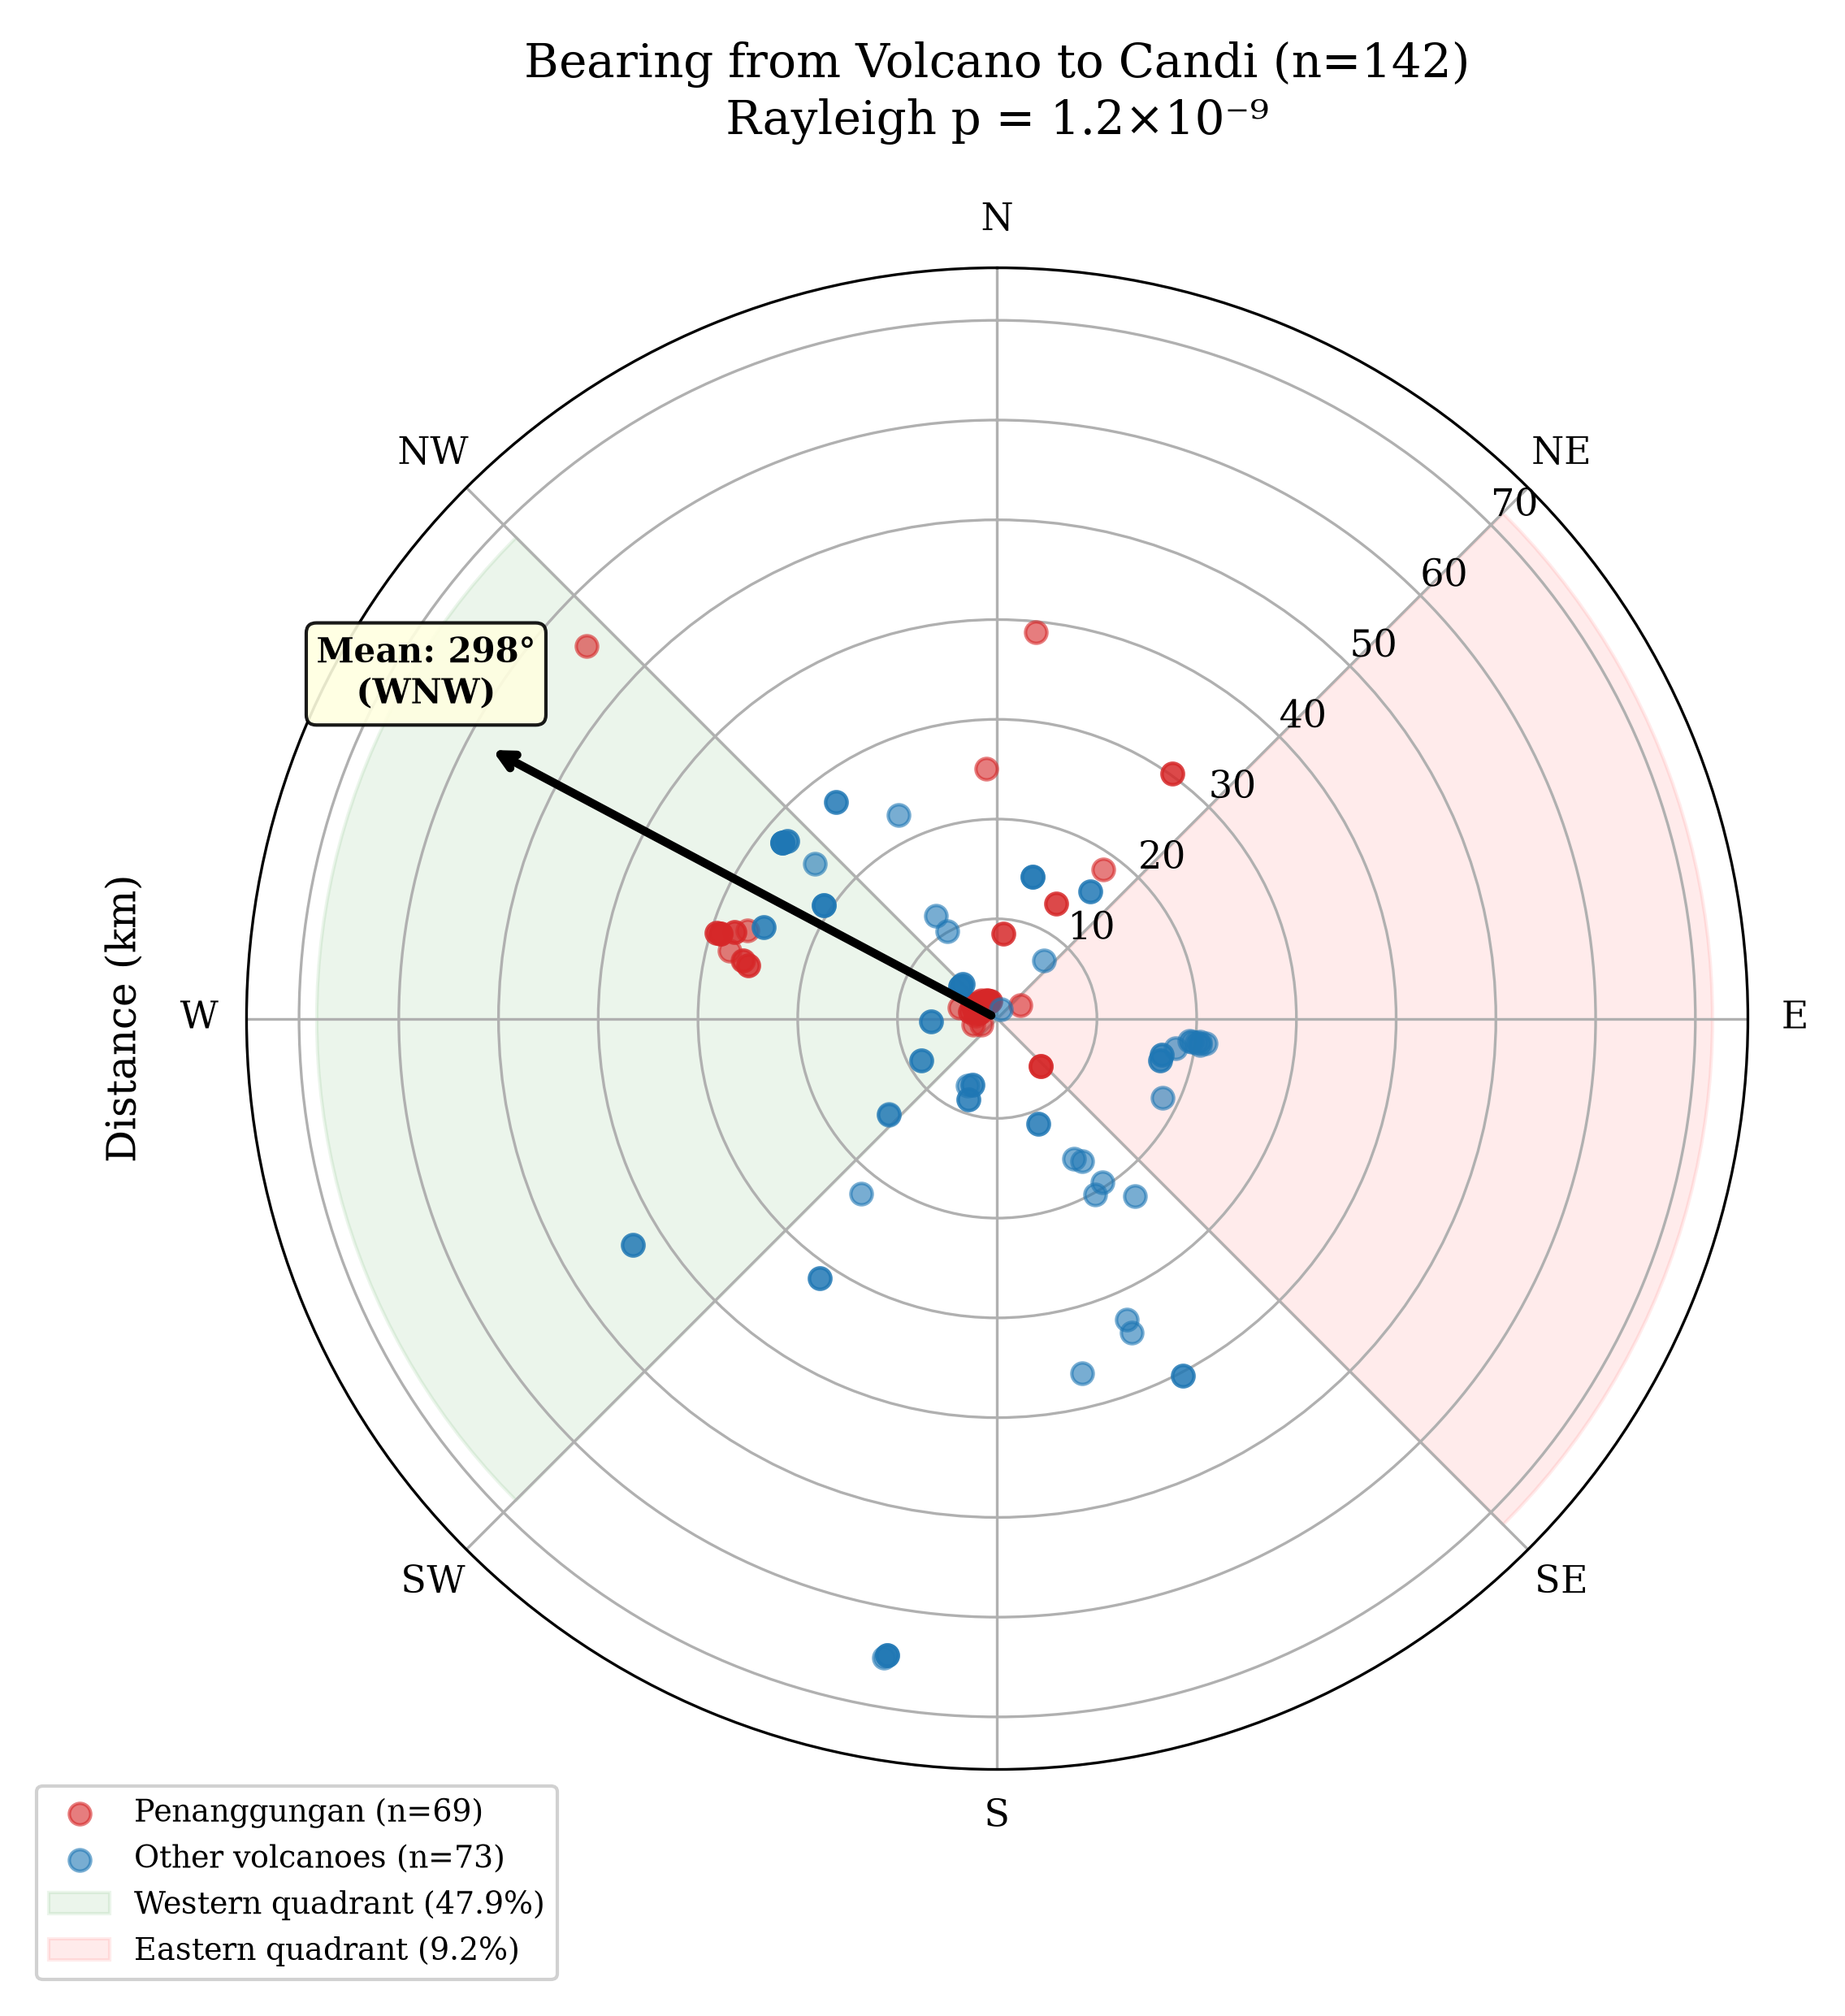
\includegraphics[width=0.7\textwidth]{figures/fig1_candi_polar_bearings.png}
\caption{Polar plot of candi bearings from nearest volcanic peak. The western clustering (mean 298\textdegree{}) is consistent with positioning downwind of prevailing dry-season winds.}
\label{fig:polar}
\end{figure}

This western concentration has both practical and cosmological dimensions.
Java's dry season is dominated by the southeast monsoon, whose winds drift eruption plumes west-northwest; the western flanks are therefore the downwind side of dry-season eruptions and receive the heaviest tephra load.
For agricultural communities this ashfall is an asset---the continuously renewed fertile soils that Mohr associated with the island's densest populations.

But the pattern also resonates with Javanese sacred geography.
In the \emph{\'{S}aiva-siddh\={a}nta} tradition that shaped Javanese temple architecture, mountains are identified with the cosmic Mount Meru, axis of the universe and abode of the gods.\footnote{Ann~R.\ Kinney, Marijke~J.\ Klokke, and Lydia Kieven, \emph{Worshipping \'{S}iva and Buddha: The Temple Art of East Java} (Honolulu: University of Hawai'i Press, 2003).}
De Groot argued that the spatial organisation of Central Javanese candi reflects a deliberate sacred landscape in which temples were positioned to maintain visual and ritual connections with volcanic peaks.
The western orientation may thus carry additional significance: in Hindu-Javanese cosmology, the west (\emph{pa\'{s}cima}) is associated with Varun\d{a}, the waters, and the setting sun---an appropriate direction for funerary and ancestral candi.

De Groot's analysis of Central Javanese candi demonstrated that temples were not merely placed near volcanoes but positioned to maintain specific visual relationships with volcanic peaks---what she termed ``intervisibility'' between sacred structure and mountain summit.\footnote{De Groot, \emph{Candi, Space and Landscape}, chap.~5--6.}
Kinney, Klokke, and Kieven have shown that the iconographic programs of East Javanese temples encode directional cosmology: relief narratives progress in specific sequences around the building, calibrated to the cardinal orientation of the entrance.\footnote{Kinney, Klokke, and Kieven, \emph{Worshipping \'{S}iva and Buddha}, 42--68.}
The convergence of cosmological prescription (how temples face) and landscape pragmatism (where temples stand) suggests that the builders operated within a tradition that integrated religious knowledge with empirical observation of volcanic hazard---a tradition whose depth we can measure spatially even if its textual record has been lost.

The proximity pattern is equally revealing (Figure~\ref{fig:penanggungan}).
Zone A (within 10~km of a volcanic peak) contains 45.1\% (64 of 142) of all candi---an overrepresentation of 19.1$\times$ relative to land area.
Penanggungan alone hosts 73 candi, 63\% on its western flank.
But the pattern is not dependent on this single mountain: after excluding Penanggungan entirely, the remaining 69 candi across Java still show significant western clustering.\footnote{Excluding Penanggungan: $p = 0.0009$, confirming that the pattern is island-wide.}

\begin{figure}[h]
\centering
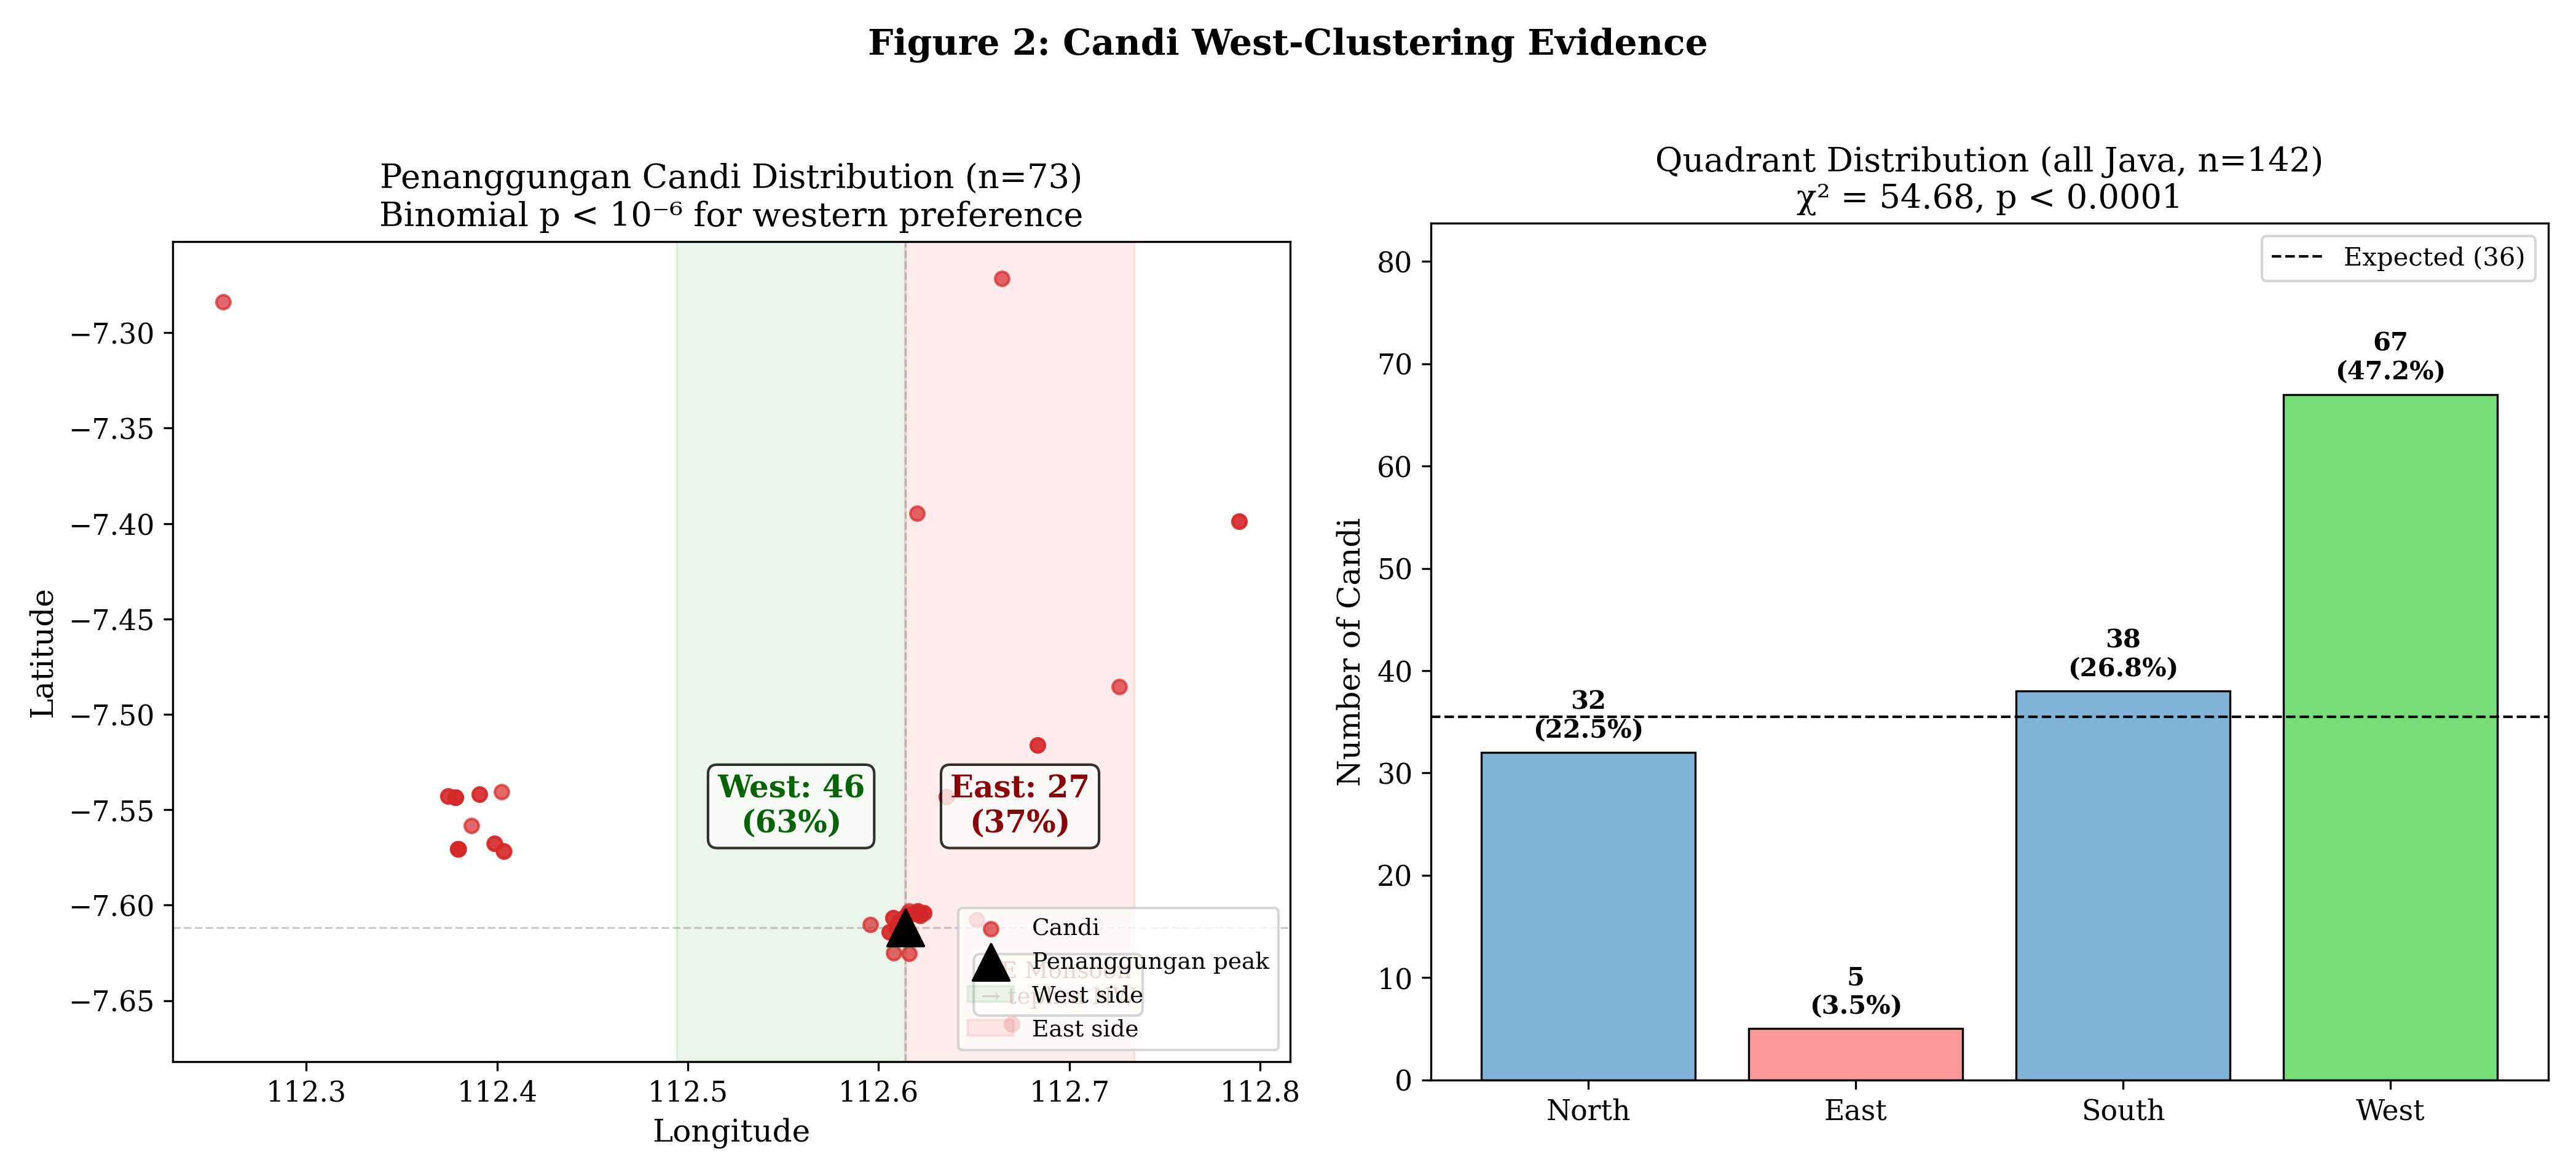
\includegraphics[width=0.7\textwidth]{figures/fig2_penanggungan_westclustering.png}
\caption{Distribution of 73 candi on Mount Penanggungan, showing the western-flank concentration. The pattern persists across Java after this mountain is excluded.}
\label{fig:penanggungan}
\end{figure}

\subsection{Orientation Follows Canon, Siting Follows Landscape}

A critical distinction emerges when we examine not where candi were placed but how they were oriented.
Of the 20 candi for which entrance orientations are recorded in published surveys---only 14\% of the full dataset, reflecting the incomplete state of architectural documentation---85\% face the equinox direction (east or west), consistent with religious prescription in the \emph{\'{S}ilpa\'{s}\={a}stra} architectural tradition.\footnote{Binomial test: $p = 4.9 \times 10^{-14}$. The small $n$ reflects documentation gaps rather than selection; all candi with published orientations were included.}
Only 35\% face toward the nearest volcano---indistinguishable from random expectation.

The builders of Java's temples thus operated according to two distinct logics simultaneously: a textual canon governing how temples should face, and an empirical understanding of volcanic geography governing where they should stand.
This dual intentionality is what makes the candi distribution informative.
It is not random scatter but a deliberate spatial record of where communities chose to build, shaped by both religious knowledge and landscape experience.


% ============================================================
\section{The Inscription Contrast: Two Geographies of Power}
% ============================================================

\subsection{Sacred and Administrative Space}

If candi proximity to volcanoes merely reflected general settlement geography, we would expect inscriptions---which record administrative activity across the inhabited landscape---to show a similar spatial distribution.
We georeferenced 182 inscriptions from the DHARMA epigraphic database,\footnote{DHARMA project, \emph{The Domestication of ``Hindu'' Asceticism and the Religious Making of South and Southeast Asia: Epigraphic Database} (CNRS/ERC, 2024), \url{https://dharma.hypotheses.org/}.} of which the 175 located on Java and Bali form the analysis set, re-derived against the canonical 30-volcano inventory.

The contrast is stark.
Inscriptions are on average 6.1~km farther from volcanoes than candi.\footnote{Mann-Whitney $U$ test: $p = 2.8 \times 10^{-7}$.}
While 45.1\% of candi lie in Zone A (within 10~km of a volcano), only 13.1\% of inscriptions do.
Inscriptions instead cluster in what we term the ``court zone'' (15--30~km from volcanoes), on the fertile alluvial plains where the Kedu, Prambanan, and Brantas polities established their administrative centres.

This spatial divergence is not a statistical artefact.
It reflects a fundamental distinction between two modes of cultural production.
Candi are architectural, devotional, and landscape-embedded---expressions of the relationship between communities and their sacred mountains.
Inscriptions are textual, administrative, and court-produced---records of \emph{sima} (tax-free) land grants, royal genealogies, and boundary demarcations in Sanskrit formulaic prose.\footnote{On the institutional character of Javanese inscriptions, see de Casparis, \emph{Indonesian Palaeography}, 15--42.}
These two genres of evidence were produced by different institutions, for different purposes, in systematically different locations.

This has consequences for archaeological inference.
Scholars have routinely used inscription counts as proxies for population density, political complexity, or the reach of ``Indianization.''\footnote{George Coed\`{e}s, \emph{The Indianized States of Southeast Asia}, trans.\ Susan Brown Cowing (Honolulu: University of Hawai'i Press, 1968).}
But if inscriptions are a court technology concentrated in a specific geographic zone, then inscription-based estimates systematically overrepresent the Sanskritized court world and underrepresent the indigenous volcanic-slope world where most of Java's population likely lived.

\subsection{The 929~CE Discontinuity}

The political migration from Central to East Java in 929~CE provides a before-after observation that illuminates this spatial structure.
The causes of the Mataram collapse remain debated---Merapi eruptions, political conflict, economic reorganisation---but the consequences for the inscriptional record are well documented.\footnote{Jan Wisseman Christie, ``Revisiting early Mataram,'' in \emph{Fruits of Inspiration: Studies in Honour of Prof.\ J.G.\ de Casparis}, ed.\ Marijke~J.\ Klokke and Karel~R.\ van Kooij (Groningen: Egbert Forsten, 2001), 25--55. See also Kenneth~R.\ Hall, \emph{A History of Early Southeast Asia: Maritime Trade and Societal Development, 100--1500} (Lanham: Rowman \& Littlefield, 2011).}

Before 929~CE, 58\% of dated and georeferenced inscriptions ($n=100$) are located in the court zone, and 91\% of those court-zone inscriptions are Sanskrit-dominant.
After 929, 48\% ($n=31$) appear in the periphery ($>$30~km from volcanoes), and 87\% of those are mixed or indigenous-rich in vocabulary.\footnote{Percentages re-derived 2026-08-13 on the canonical 30-volcano inventory (E105 canonical-30 re-run); the earlier partial-inventory run gave 57/91/53/89\%.}

This shift has traditionally been interpreted as ``de-Indianization'' or ``Javanization''---a civilisation-wide retreat from Indic cultural forms.\footnote{On the Indianization debate and its critiques, see Hermann Kulke, ``Indian Colonies, Indianization or Cultural Convergence?,'' in \emph{Unterwegs nach Indien}, ed.\ H.\ Becker and R.\ Ptak (Munich: Museum f\"{u}r V\"{o}lkerkunde, 1990). Sheldon Pollock, \emph{The Language of the Gods in the World of Men: Sanskrit, Culture, and Power in Premodern India} (Berkeley: University of California Press, 2006).}
But the spatial data suggest a more precise interpretation: what changed at 929~CE was not Javanese culture but the \emph{geography of textual production}.
The court system that had generated Sanskrit inscriptions in the 15--30~km zone collapsed.
Epigraphic activity migrated to the periphery, where indigenous vocabulary had always been the norm.

If this interpretation is correct, the ``de-Indianization'' narrative may describe a change in \emph{who was writing inscriptions and where}, rather than a transformation of Javanese cultural identity.
In Wolters' terms, the indigenous substrate was never absent---it was merely invisible within the court zone's inscriptional genre.
The 929~CE collapse removed the Sanskrit overlay and revealed the underlying cultural landscape.

Christie's influential analysis of demographic trends in early Java reinforces this interpretation from a different angle.
Her ``states without cities'' argument held that early Javanese polities were not urban in any conventional sense: political power was exercised through dispersed control of wet-rice agricultural production, not through concentrated urban populations.\footnote{Jan Wisseman Christie, ``States without Cities: Demographic Trends in Early Java,'' \emph{Indonesia} 52 (1991): 23--40.}
If the population was dispersed across the agrarian landscape rather than concentrated in administrative centres, then inscription-based estimates of settlement density---which are anchored to court locations---systematically misrepresent where people actually lived.
The Two Javas model provides the spatial correlate to Christie's demographic argument: the court zone produced the texts, but the volcano zone housed the villages.


% ============================================================
\section{Liangan: A Window into the Buried Landscape}
% ============================================================

The discovery of Liangan in 2008 provides the most direct illustration of the model's plausibility.
Located 5.5~km from Mount Sindoro on its western flank---Zone A, western quadrant---the site was found not by archaeologists but by sand miners, who exposed a complete Mataram-era settlement beneath 4--6~m of pyroclastic deposits.\footnote{Novida Abbas, ed., \emph{Liangan: Mozaik Peradaban Mataram Kuno di Lereng Sindoro} (Yogyakarta: Kepel Press / Balai Arkeologi Yogyakarta, 2016).}

What Liangan preserved is precisely what our analysis predicts should exist but cannot be detected by surface survey: wooden houses with post-hole foundations, carbonised rice grains (\emph{tropical japonica}), an iron-smelting workshop with slag and tuyères, Tang Dynasty ceramics indicating long-distance trade networks, and the complete domestic infrastructure of a Hindu-Buddhist-era village.
The site yielded both a Hindu temple (Candi Liangan) and the village that surrounded it---the combination that our model posits for every known candi but that volcanic burial has rendered invisible elsewhere.

The closest analogue is Cerén in El Salvador, the Central American village sealed by a single eruption c.~600~CE that preserved sleeping mats, stored food, and agricultural tools.\footnote{Payson~D.\ Sheets, ed., \emph{Before the Volcano Erupted: The Ancient Cer\'{e}n Village in Central America} (Austin: University of Texas Press, 2002).}
Both sites demonstrate that volcanic burial can preserve the vernacular layer of pre-modern life that normally leaves no archaeological trace.
But where Cerén resulted from a single catastrophic event, Liangan was buried by cumulative deposition over centuries---the process that characterises Java's volcanic taphonomy more broadly.

Liangan is not an anomaly but a proof of possibility.
If the spatial patterns identified in this paper are correct, similar sites lie beneath the volcanic deposits of East Java's western flanks, awaiting discovery---or destruction by unmonitored mineral extraction.


% ============================================================
\section{Heritage Implications: What is Being Lost}
% ============================================================

The practical urgency of these findings lies in the ongoing destruction of potential archaeological sites by sand and gravel mining on volcanic slopes.
Liangan was discovered by miners.
But for every site exposed and reported, others are likely destroyed without documentation.
The western flanks of East Java's volcanoes---where our model predicts the highest concentration of buried sites---are precisely the zones targeted for mineral extraction due to the abundance of volcanic aggregate.

Indonesia's rescue archaeology capacity is minimal by international standards: approximately 70 excavations per year, compared to Japan's 8,300.\footnote{Hiroki Takata and Takahiro Yanase, ``Production, Preservation and Dissemination of Archaeological Data in Japan,'' \emph{Internet Archaeology} 58 (2022).}
The mechanisms by which buried sites become known elsewhere---developer-funded excavation, systematic geophysical survey, ground-penetrating radar reconnaissance\footnote{Lawrence~B.\ Conyers, \emph{Ground-Penetrating Radar for Archaeology} (Walnut Creek: AltaMira Press, 2004).}---have not been deployed at scale in Indonesian volcanic zones.

The spatial model developed here identifies ten priority areas for geophysical survey, derived from the intersection of candi clustering, terrain suitability, and sedimentation rate estimates.
These coordinates are available to authorised heritage bodies (BPCB, Balai Arkeologi) upon request.
The most productive survey depths---2 to 9~m, based on colonial-era burial data and the Liangan precedent---are within the range of electrical resistivity tomography and ground-penetrating radar.

What is at stake is not merely archaeological curiosity but the recovery of a \emph{monde insulindien} that Lombard intuited but could not yet document: the vernacular landscape of pre-modern Java, hidden beneath the volcanic soils that sustained it.

The current evidential gap has institutional as well as geological roots.
As Bloembergen and Eickhoff have documented, the colonial \emph{Oudheidkundige Dienst} constructed its archaeological priorities around monumental Hindu-Buddhist remains---candi, inscriptions, relief panels---that served the colonial narrative of a pre-Islamic ``golden age.''\footnote{Marieke Bloembergen and Martijn Eickhoff, \emph{The Politics of Heritage in Indonesia: A Cultural History} (Cambridge: Cambridge University Press, 2020), esp.\ chap.~2--4 on colonial archaeological priorities and their postcolonial persistence.}
Vernacular sites---villages, workshops, agricultural infrastructure---were neither sought nor recorded.
This institutional bias persists in postcolonial heritage management, where the \emph{Balai Pelestarian Cagar Budaya} (BPCB) focuses on registered monuments rather than systematic landscape survey.
The geological erasure of the volcanic-slope settlement record has thus been compounded by an institutional erasure that privileges the monumental over the domestic.


% ============================================================
\section{Discussion: The Buried Crossroads}
% ============================================================

The convergence of these evidence lines---candi clustering on western volcanic flanks, the inscription-architecture divergence, documented burial depths of 3--9~m, the Liangan discovery, and the survey-intensity control---points toward a single conclusion: pre-modern Java was far more extensively settled in volcanic zones than the surviving record indicates.

A potential objection is that the archaeological gap near volcanoes reflects differential survey effort rather than genuine burial.
We tested this using robustness regression controlling for three survey-intensity proxies (road distance, proximity to heritage offices, university proximity).
After controlling for all three, volcanic proximity still explains additional variance in site counts.\footnote{Quasi-Poisson GLM on the canonical 30-volcano Java inventory: volcanic proximity $\beta = -0.831$, likelihood-ratio $p = 2.9 \times 10^{-7}$ (dispersion-adjusted quasi-likelihood). The signal strengthens relative to the earlier 7-volcano run ($\beta = -0.477$, $p = 0.0015$).}
The deficit is real, not a survey artefact.

What this means is that the monumental record we possess---the candi, the inscriptions, the literary texts---represents only the fraction of Javanese civilisation that happened to be encoded in durable media \emph{and} located at distances or depths where survival was possible.
The vernacular layer---the houses, the markets, the workshops, the rice granaries---has been systematically subtracted from the evidential base.
Lombard's ``Javanese crossroads'' is therefore not merely a crossroads of cultures but a \emph{buried} crossroads, whose full spatial extent remains to be excavated.

The 71\% temple bias in East Java's archaeological database---where candi account for the vast majority of known sites, while settlements represent barely 1\%---further illustrates the distortion.\footnote{Of 391 known archaeological sites in East Java, 277 (70.8\%) are temples or temple fragments; with statues and inscriptions, monuments account for 73.1\%. Only 5 (1.3\%) are identified settlements.}
This is not a reflection of past reality but of what survives: stone resists, wood does not.
The spatial patterns identified here suggest where the missing settlements might be found.

\subsection{Limitations}

The Penanggungan concentration (51\% of all candi) limits spatial generalisability, though the pattern survives its exclusion.
All evidence remains indirect---no subsurface geophysical validation has yet been conducted.
The temporal range of the candi proxy (c.~8th--15th century) does not extend to the pre-Hindu or Islamic periods.
The geocoding of inscriptions carries a mean uncertainty of $\pm$5~km for some entries, which may blur zone boundaries.
Finally, the argument rests on the assumption that candi and their associated settlements were co-located---an assumption supported by the candi-settlement proximity test but not yet confirmed by excavation.
Crucially, the model generates testable predictions: ground-penetrating radar and electrical resistivity survey of ten western-flank sites at 2--9~m depth should yield buried settlement remains.
If systematic geophysical survey finds nothing at predicted locations, the model would be refuted---a condition that distinguishes this framework from unfalsifiable post-hoc narrative.


% ============================================================
\section{Conclusion}
% ============================================================

The temples of Java stand as markers of a civilisation far larger than what survives on the surface.
By reading their spatial distribution---not as a catalogue of monuments but as a map of past communities---we can begin to reconstruct the settlement geography that volcanic sedimentation has erased.

Two distinct landscapes of cultural production emerge from this analysis: a sacred landscape on volcanic slopes, where communities built temples in dialogue with the mountain cosmology that structured their religious life; and an administrative landscape on the alluvial plains, where courts generated the inscriptional record from which historians have reconstructed ``Javanese civilisation.''
The 929~CE Mataram collapse, by removing the court system that had generated Sanskrit-heavy inscriptions, revealed an indigenous cultural substrate that had been present throughout---hidden not by its own absence but by the genre conventions of court epigraphy.

This is not merely a methodological contribution.
It is a reframing of how we understand the archaeological record of the \emph{monde insulindien}'s most volcanically active island.
The silence in the record is not evidence of absence; it is evidence of burial.
And the temples, paradoxically, are both survivors of that process and guides to what lies beneath.

\vspace{1em}
\noindent\textbf{AI Disclosure.} This research used AI tools (Claude, Anthropic) for spatial geocoding, statistical computation, and manuscript drafting assistance. All statistical analyses were independently verified using standard libraries (SciPy, GeoPandas). Research design, hypothesis formation, data interpretation, and all conclusions are the authors' work. Code and data are available at the project repository.


% ============================================================
\section*{Bibliography}
% ============================================================

\noindent Abbas, Novida, ed.\ \emph{Liangan: Mozaik Peradaban Mataram Kuno di Lereng Sindoro}. Yogyakarta: Kepel Press / Balai Arkeologi Yogyakarta, 2016.

\vspace{0.5em}
\noindent Bloembergen, Marieke, and Martijn Eickhoff. \emph{The Politics of Heritage in Indonesia: A Cultural History}. Cambridge: Cambridge University Press, 2020.

\vspace{0.5em}
\noindent de Casparis, J.~G.\ \emph{Indonesian Palaeography: A History of Writing in Indonesia from the Beginnings to c.~A.D.~1500}. Leiden: E.~J.\ Brill, 1975.

\vspace{0.5em}
\noindent Christie, Jan Wisseman. ``States without Cities: Demographic Trends in Early Java.'' \emph{Indonesia} 52 (1991): 23--40.

\vspace{0.5em}
\noindent Christie, Jan Wisseman. ``Revisiting Early Mataram.'' In \emph{Fruits of Inspiration: Studies in Honour of Prof.~J.G.\ de Casparis}, edited by Marijke~J.\ Klokke and Karel~R.\ van Kooij, 25--55. Groningen: Egbert Forsten, 2001.

\vspace{0.5em}
\noindent Coed\`{e}s, George. \emph{The Indianized States of Southeast Asia}. Translated by Susan Brown Cowing. Honolulu: University of Hawai'i Press, 1968.

\vspace{0.5em}
\noindent Conyers, Lawrence~B.\ \emph{Ground-Penetrating Radar for Archaeology}. Walnut Creek: AltaMira Press, 2004.

\vspace{0.5em}
\noindent de Groot, V\'{e}ronique~M.Y.\ \emph{Candi, Space and Landscape: A Study on the Distribution, Orientation and Spatial Organization of Central Javanese Temple Remains}. PhD diss., Leiden University, 2009.

\vspace{0.5em}
\noindent DHARMA project. \emph{The Domestication of ``Hindu'' Asceticism and the Religious Making of South and Southeast Asia: Epigraphic Database}. CNRS/ERC, 2024. \url{https://dharma.hypotheses.org/}.

\vspace{0.5em}
\noindent Dumar\c{c}ay, Jacques. \emph{The Temples of Java}. Oxford: Oxford University Press, 1993.

\vspace{0.5em}
\noindent Global Volcanism Program. \emph{Volcanoes of the World}. V.~5.1.1. Smithsonian Institution, 2023. \url{https://volcano.si.edu/}.

\vspace{0.5em}
\noindent Hall, Kenneth~R.\ \emph{A History of Early Southeast Asia: Maritime Trade and Societal Development, 100--1500}. Lanham: Rowman \& Littlefield, 2011.

\vspace{0.5em}
\noindent Kinney, Ann~R., Marijke~J.\ Klokke, and Lydia Kieven. \emph{Worshipping \'{S}iva and Buddha: The Temple Art of East Java}. Honolulu: University of Hawai'i Press, 2003.

\vspace{0.5em}
\noindent Kulke, Hermann. ``Indian Colonies, Indianization or Cultural Convergence? Reflections on the Changing Image of India's Role in South-East Asia.'' In \emph{Unterwegs nach Indien}, edited by H.\ Becker and R.\ Ptak. Munich: Museum f\"{u}r V\"{o}lkerkunde, 1990.

\vspace{0.5em}
\noindent Lavigne, Franck, and Jean-Claude Thouret. ``Sediment Transportation and Deposition by Rain-Triggered Lahars at Merapi Volcano, Central Java, Indonesia.'' \emph{Geomorphology} 49, no.~1--2 (2003): 45--69.

\vspace{0.5em}
\noindent Lombard, Denys. \emph{Le carrefour javanais: essai d'histoire globale}. 3 vols. Paris: \'{E}ditions de l'\'{E}cole des hautes \'{e}tudes en sciences sociales, 1990.

\vspace{0.5em}
\noindent Miksic, John~N.\ ``The Classical Cultures of Indonesia.'' In \emph{Southeast Asia: From Prehistory to History}, edited by Ian Glover and Peter Bellwood, 234--256. London: RoutledgeCurzon, 2004.

\vspace{0.5em}
\noindent Mohr, E.~C.~J.\ ``The Relation between Soil and Population Density in the Netherlands East Indies.'' In \emph{Comptes Rendus du Congr\`{e}s International de G\'{e}ographie}. Amsterdam, 1938.

\vspace{0.5em}
\noindent Newhall, Christopher~G., et al.\ ``10,000 Years of Explosive Eruptions of Merapi Volcano, Central Java: Archaeological and Modern Implications.'' \emph{Journal of Volcanology and Geothermal Research} 100, no.~1--4 (2000): 9--50.

\vspace{0.5em}
\noindent \emph{Oudheidkundig Verslag}. Batavia: Oudheidkundige Dienst in Nederlandsch-Indi\"{e}, 1912--1929.

\vspace{0.5em}
\noindent Pollock, Sheldon. \emph{The Language of the Gods in the World of Men: Sanskrit, Culture, and Power in Premodern India}. Berkeley: University of California Press, 2006.

\vspace{0.5em}
\noindent Putra, Prishardoyo Bagyo, and Ayu Setyastuti. ``Le complexe cultuel de Kimpulan, site enfoui sous les cendres du Merapi (Yogyakarta, Java central).'' \emph{Bulletin de l'\'{E}cole fran\c{c}aise d'Extr\^{e}me-Orient} 105 (2019): 377--402.

\vspace{0.5em}
\noindent Schiffer, Michael~B.\ \emph{Formation Processes of the Archaeological Record}. Albuquerque: University of New Mexico Press, 1987.

\vspace{0.5em}
\noindent Sheets, Payson~D., ed.\ \emph{Before the Volcano Erupted: The Ancient Cer\'{e}n Village in Central America}. Austin: University of Texas Press, 2002.

\vspace{0.5em}
\noindent Soekmono, R.\ \emph{The Javanese Candi: Function and Meaning}. Leiden: Brill, 1995.

\vspace{0.5em}
\noindent Takata, Hiroki, and Takahiro Yanase. ``Production, Preservation and Dissemination of Archaeological Data in Japan.'' \emph{Internet Archaeology} 58 (2022).

\vspace{0.5em}
\noindent van Bemmelen, R.~W.\ \emph{The Geology of Indonesia}. Vol.~1A. The Hague: Government Printing Office, 1949.

\vspace{0.5em}
\noindent Whitten, Tony, Roehayat Emon Soeriaatmadja, and Suraya~A.\ Afiff. \emph{The Ecology of Java and Bali}. Singapore: Periplus Editions, 1996.

\vspace{0.5em}
\noindent Wolters, O.~W.\ \emph{History, Culture, and Region in Southeast Asian Perspectives}. Rev.\ ed. Ithaca: Cornell University Southeast Asia Program, 1999.

\end{document}
